% !TEX program = pdflatex -> bibtex -> pdflatex*2
\documentclass{assignment}
\ProjectInfos{量子力学}{PHYS1501}{2020-2021学年第一学期}{第一次作业}{截止时间:2020. 09. 08(周二)}{陈润植}[https://github.com/Chen-Jialin]{45875852}

\begin{document}
    \begin{prob}
        请证明本 \LaTeX 模板支持以下功能:
        \begin{itemize}
            \item[(1)] 数学公式;
            \item[(2)] 化学反应方程式.
            % \item[(3)] 量子线路图.
        \end{itemize}
    \end{prob}
    \begin{pf}
        \begin{itemize}
            \item[(1)] 三维空间中,位于位势$V(\bm{r},t)$中的单粒子薛定谔方程为
            \begin{equation}
                i\hbar\frac{\partial}{\partial t}\lvert\psi(\bm{r},t)\rangle=-\frac{\hbar^2}{2m}\nabla^2\lvert\psi(\bm{r},t)\rangle+V(\bm{r},t)\lvert\psi(\bm{r},t)\rangle.
            \end{equation}
            \item[(2)] 加热并用浓硫酸催化,苯可与硝酸反应生成硝基苯:
            % 在线工具:https://py-chemist.com/mol_2_chemfig/home
            \begin{equation}
                \ce{\chemfig{*6([,.5]-=-=-=)} + \chemfig{[,.75]HO-NO_2} ->[\mbox{浓硫酸}][$\Delta$] \chemfig{*6([,.5]-=-(-NO_2)=-=)} + H2O}
            \end{equation}
            % \item[(3)] 量子傅里叶变换的线路图为
            % \begin{center}
            %     \begin{quantikz}
            %         \lstick{$q_0$} & \gate{H} & \gate{\begin{array}{c}P\\\pi/8\end{array}} & \gate{\begin{array}{c}P\\\pi/4\end{array}} & \gate{\begin{array}{c}P\\\pi/2\end{array}} & \qw & \qw & \qw & \qw & \qw & \qw & \qw\\
            %         \lstick{$q_1$} & \qw & \qw & \qw & \ctrl{-1} & \gate{H} & \gate{\begin{array}{c}P\\\pi/4\end{array}} & \gate{\begin{array}{c}P\\\pi/2\end{array}} & \qw & \qw & \qw & \qw\\
            %         \lstick{$q_2$} & \qw & \qw & \ctrl{-2} & \qw & \qw & \qw & \ctrl{-1} & \gate{H} & \gate{\begin{array}{c}P\\\pi/2\end{array}} & \qw & \qw\\
            %         \lstick{$q_3$} & \qw & \ctrl{-3} & \qw & \qw & \qw & \ctrl{-2} & \qw & \qw & \ctrl{-1} & \gate{H} & \qw
            %     \end{quantikz}
            % \end{center}
        \end{itemize}
    \end{pf}

    \clearpage
    \begin{prob}
        请完成以下操作:
        \begin{itemize}
            \item[(1)] 插入图片;
            \begin{itemize}
                \item[(a)] 单张图片,强制设定图片位置;
                \item[(b)] 两张子图;
            \end{itemize}
            \item[(2)] 插入表格,要求如下:
            \begin{itemize}
                \item[$\triangleright$] 含有多行、多列单元格合并;
                \item[$\triangleright$] 三线表;
                \item[$\triangleright$] 表格跨页;
            \end{itemize}
            \item[(3)] 插入代码;
            \item[(4)] 引用文献.
        \end{itemize}
    \end{prob}
    \begin{sol}
        \begin{itemize}
            \item[(1)]
            \begin{itemize}
                \item[(a)] 如图\ref{Lenna}.
                \begin{figure}[hbt!]
                    \centering
                    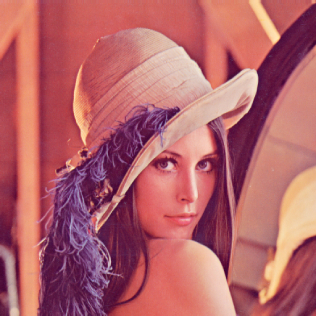
\includegraphics[width=.2\textwidth]{Lenna.jpg}
                    \caption{莱娜}
                    \label{Lenna}
                \end{figure}
                \item[(b)] 如\ref{Lenna2}中的子图\ref{lenna1}和\ref{lenna2}.
                \begin{figure}[hbt!]
                    \centering
                    \subfigure[莱娜1]{
                    \label{lenna1}
                    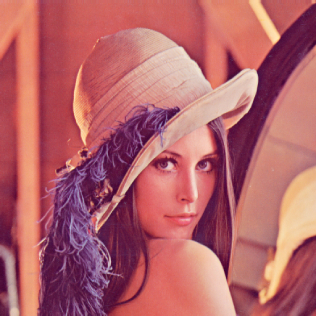
\includegraphics[width=0.2\textwidth]{Lenna.jpg}}
                    \subfigure[莱娜2]{
                    \label{lenna2}
                    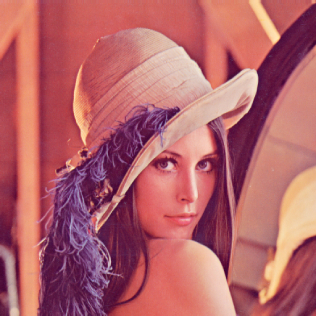
\includegraphics[width=0.2\textwidth]{Lenna.jpg}}
                    \caption{莱娜}
                    \label{Lenna2}
                \end{figure}
            \end{itemize}
            \item[(2)] 如表\ref{my-table}.
            % 在线工具:https://www.tablesgenerator.com/
            \begin{center}
                \begin{longtable}{ccccc}
                    \caption{示例表格}
                    \label{my-table}\\ \toprule
                    \multirow{2}{*}{\begin{tabular}[c]{@{}c@{}}多行单元格\\ 合并\end{tabular}} & \multicolumn{2}{c}{多列单元格合并} & \multicolumn{2}{c}{多列单元格合并} \\ \cline{2-5} 
                      & 列1 & 列2 & 列a & 列b \\ \midrule
                    如 & 迈  & 咽  & 霜  & 西  \\
                    海 & 步  & 雄  & 晨  & 风  \\
                    残 & 从  & 关  & 月  & 烈  \\
                    阳 & 头  & 漫  & 马  & 长  \\
                    如 & 越  & 道  & 蹄  & 空  \\
                    血 & 从  & 真  & 声  & 雁  \\
                      & 头  & 如  & 碎  & 叫  \\
                      & 越  & 铁  & 喇  & 霜  \\
                      & 苍  & 而  & 叭  & 晨  \\
                      & 山  & 今  & 声  & 月  \\ \bottomrule
                \end{longtable}
            \end{center}
            \item[(3)] 代码如下:
\begin{lstlisting}[language=Fortran]
program main
    implicit none

    write(*,*) 'hello world'
end program main
\end{lstlisting}
            \item[(4)] 鲁迅先生说过\cite{luxun2006}:“贪安稳就没有自由,要自由就要历些危险,只有这两条路。”
        \end{itemize}
    \end{sol}

    \bibliographystyle{unsrt}
    \bibliography{Assignment-zh}
\end{document}